\begin{tikzpicture}[
	every path/.style={line join=round,line cap=round},
	legend/.style={
		node font=\fontsize{13pt}{1em}\selectfont
	},
	fpga/.style={Tblue},
	ethcon/.style={Tred},
	phy/.style={Torange},
	marking/.style={line width=3.5pt},
	callout/.style={line width=1.5pt}
]
\node[anchor=south west,inner sep=0] (Image) at (0,0) {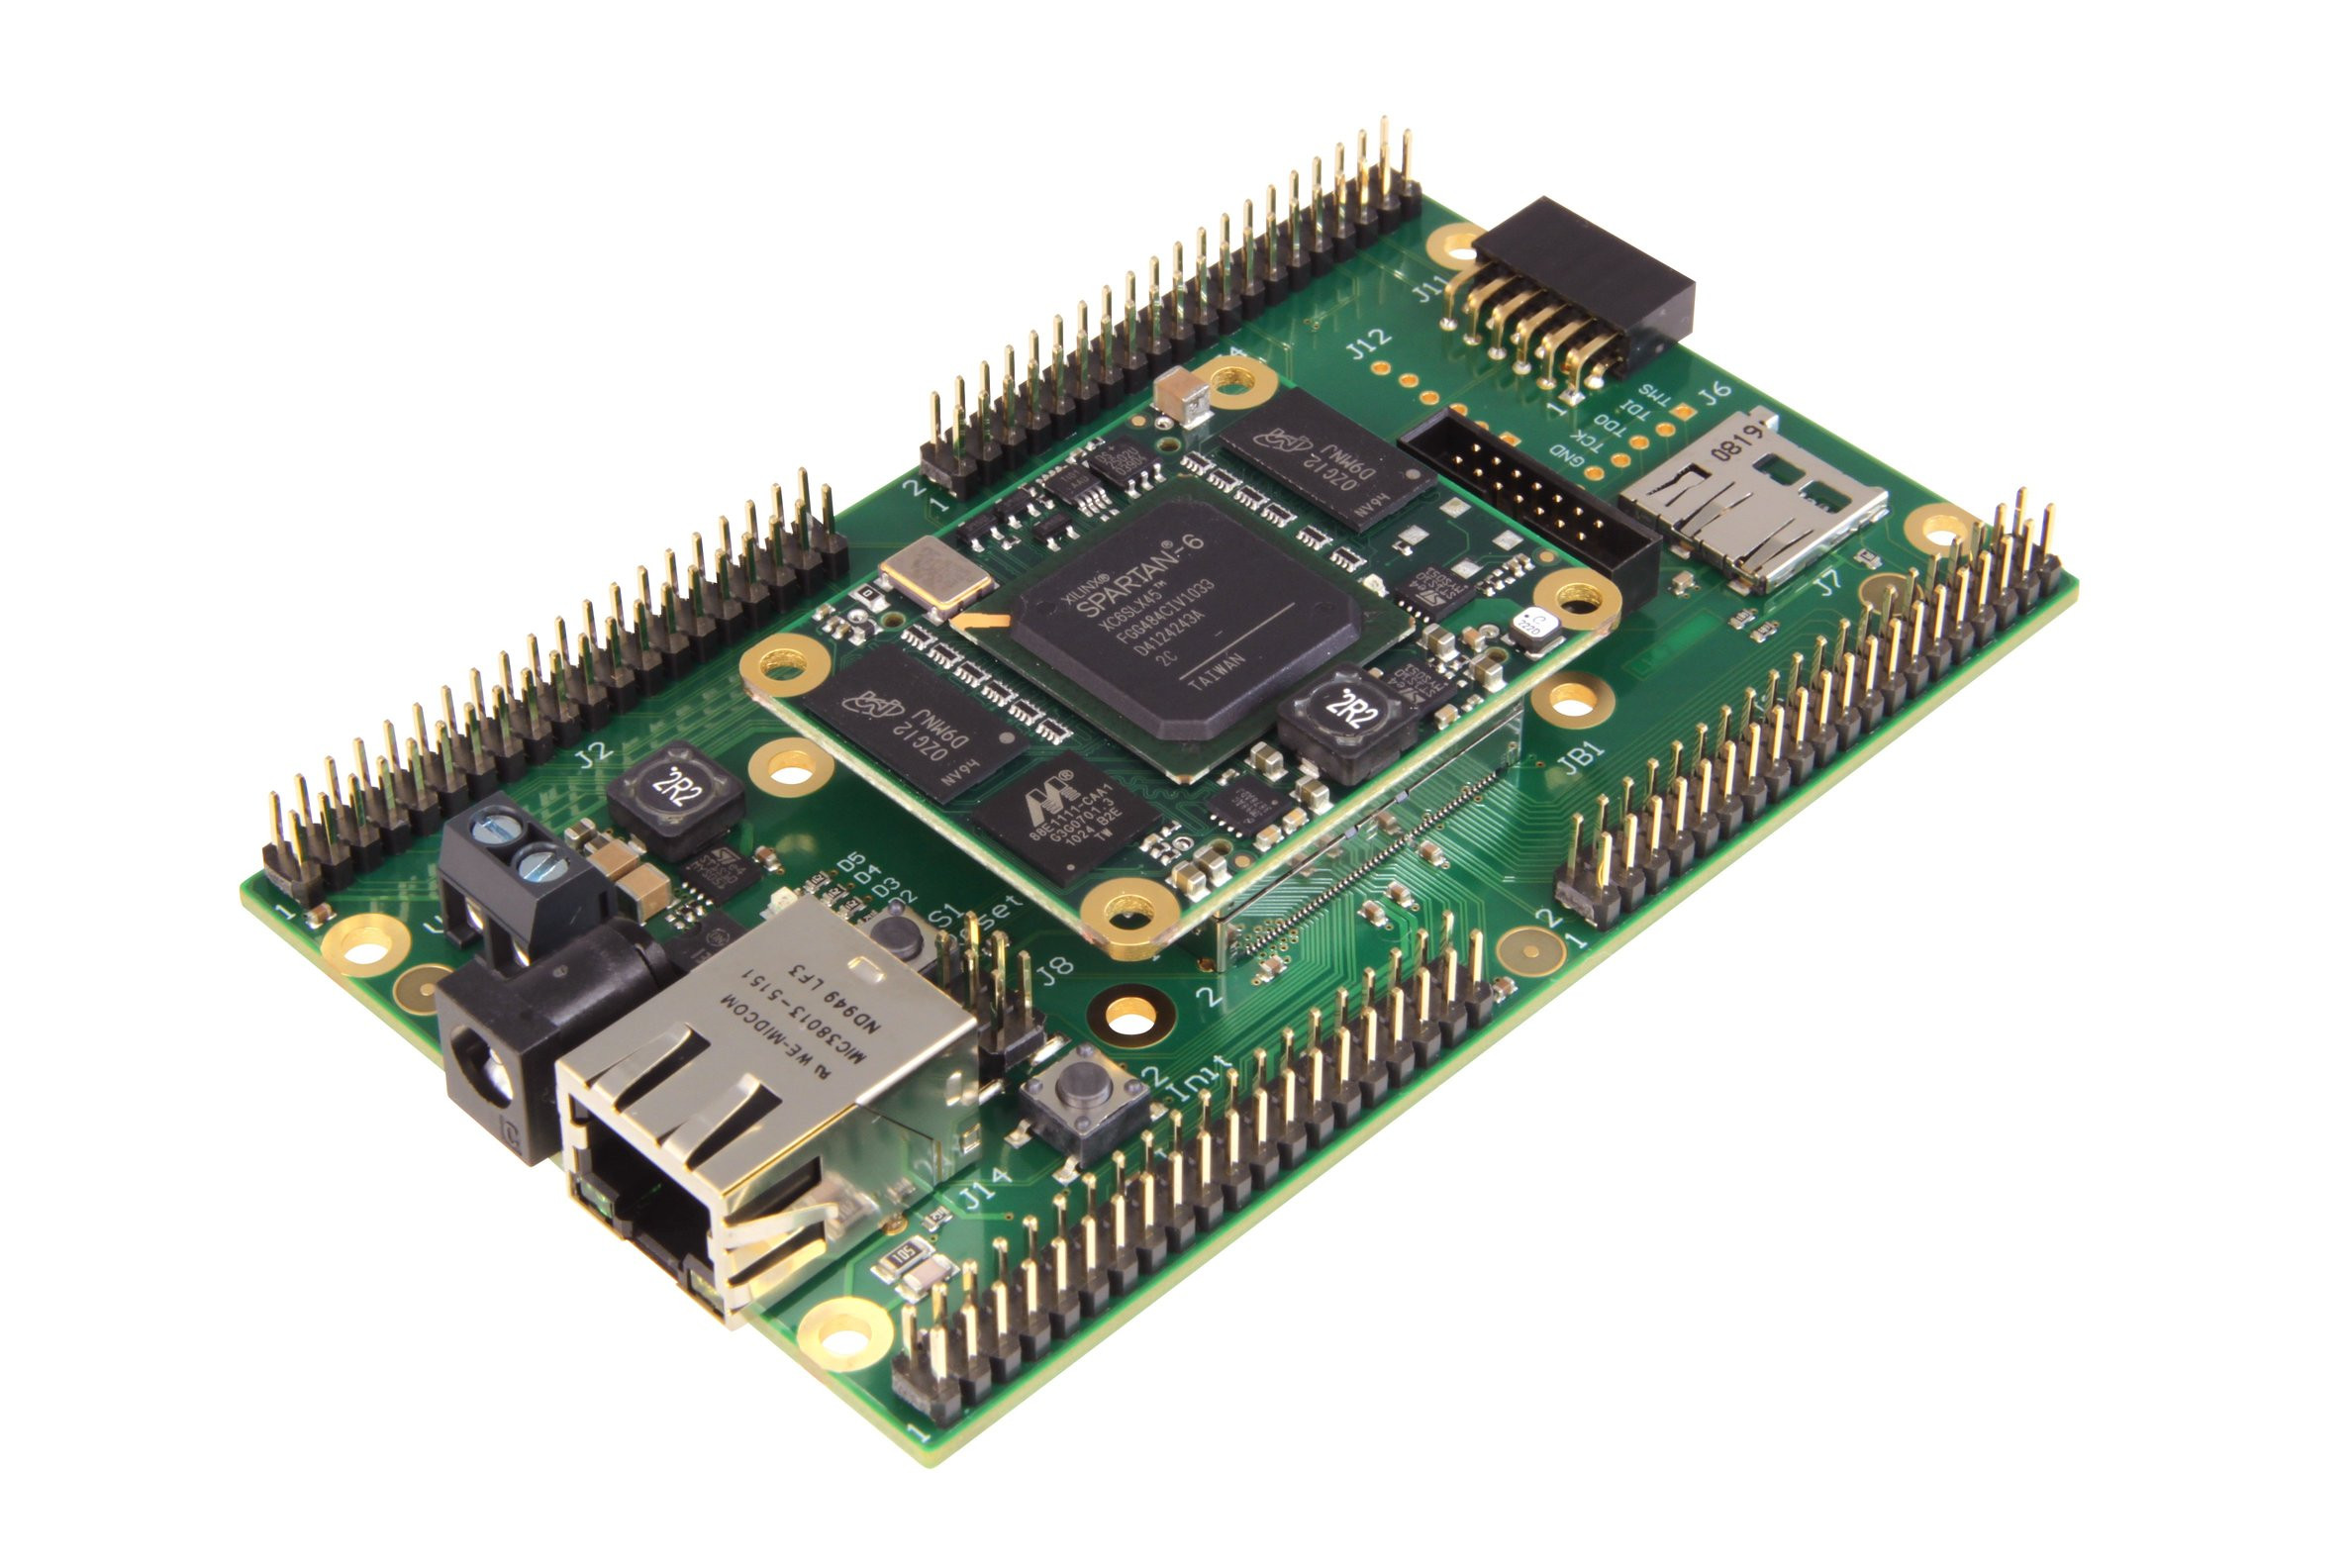
\includegraphics[width=0.8\textwidth]{Figures/TE603+TE600.angle.jpg}};
% Transform coordinate system to normal picture coordinates
\begin{scope}[x={(Image.south east)},y={(Image.north west)},yscale=-1,shift={($(Image.north) - (Image.south)$)}]
	%\draw[red,ultra thick] (0.26,0.12) rectangle (0.78,0.75);
	\node[legend,fpga] (FPGA) at (0.26,0.12) {Xilinx Spartan-6 family FPGA};
	\node[legend,ethcon,anchor=base] (EthCon) at (0.16,0.92) {Ethernet connector};
	\node[legend,phy,anchor=base] (PHY) at (0.72,0.92) {Marvell 88E1111 Ethernet PHY};
	
	\draw[marking,fpga] (0.505,0.508) -- (0.610,0.394) -- (0.505,0.293) -- (0.399,0.400) coordinate[midway] (FPGAEdge) -- cycle;
	\draw[callout,fpga] (FPGAEdge) -- (FPGA);
	\draw[marking,phy] (0.451,0.473) -- (0.498,0.521) -- (0.454,0.571) coordinate[midway] (PHYEdge) -- (0.407,0.520) -- cycle;
	\draw[callout,phy] (PHYEdge) -- (PHY);
	\draw[marking,ethcon] (0.345,0.564) -- (0.420,0.650) -- (0.421,0.742) -- (0.312,0.857) -- (0.236,0.768) coordinate[midway] (EthConEdge) -- (0.231,0.674) -- cycle;
	\draw[callout,ethcon] (EthConEdge) -- (EthCon);
\end{scope}
\end{tikzpicture}